\documentclass[10pt,a4paper]{article}
\usepackage[T1]{fontenc}
\usepackage{lmodern,amsmath,amssymb,amsthm,mathtools,microtype,geometry,enumitem,hyperref,tikz}
\geometry{left=19mm,right=19mm,top=16mm,bottom=16mm}
\hypersetup{hidelinks,pdftitle={Random Variables and Lebesgue Integration - Part 2 - Revised Study Notes}}
\setlength{\parindent}{0pt}\setlength{\parskip}{3.3pt}
\setlist[itemize]{topsep=4pt,itemsep=3pt}
\newtheorem{proposition}{Proposition}
\newcommand{\R}{\mathbb R}\newcommand{\Q}{\mathbb Q}\newcommand{\E}{\mathbb E}\newcommand{\B}{\mathcal B}
\begin{document}
\begin{center}
{\Large\bfseries PART 2: Random Variables and Integration}\par
{\normalsize Mathematical reading notes --- revised edition, 2026}
\end{center}
\vspace{8pt}
\textbf{Topics.} Measurable functions (\S3.2), random variables (\S3.5), their laws (\S3.6), nonnegative Lebesgue integrals and monotone convergence (\S4.2), signed integrals and dominated convergence (\S4.3), and expectation (\S4.4).

\section*{1. Measurable functions (\S3.2)}
Let $(S_1,\mathcal S_1)$ and $(S_2,\mathcal S_2)$ be measurable spaces. A function $f:S_1\to S_2$ is measurable when
\[
f^{-1}(B)\in\mathcal S_1\qquad\text{for every }B\in\mathcal S_2.
\]
The condition concerns \emph{preimages}, not images: taking the preimage of every measurable target set must give a measurable subset of the domain. This is also called $\mathcal S_1/\mathcal S_2$ measurability.

\subsection*{Example: indicator functions}
For $A\in\mathcal S$, the indicator $\mathbf1_A:S\to\R$ is defined by $\mathbf1_A(x)=1$ when $x\in A$ and $0$ otherwise. For any Borel set $B\subset\R$, its preimage is one of the measurable sets
\[
\mathbf1_A^{-1}(B)=
\begin{cases}
\varnothing,&0\notin B,\ 1\notin B,\\
A^c,&0\in B,\ 1\notin B,\\
A,&0\notin B,\ 1\in B,\\
S,&0\in B,\ 1\in B.
\end{cases}
\]
Thus indicator functions of measurable sets are measurable.

\subsection*{Generators of sigma-algebras}
For a family $\mathcal C\subseteq\mathcal P(S)$, write
\[
\sigma(\mathcal C)=\bigcap\{\mathcal A:\mathcal A\text{ is a sigma-algebra on }S,
\ \mathcal C\subseteq\mathcal A\}.
\]
It is the smallest sigma-algebra containing $\mathcal C$. For example, if $S=\{1,2,3\}$ and $\mathcal C=\{\{1\}\}$, then
\[
\sigma(\mathcal C)=\{\varnothing,\{1\},\{2,3\},S\}.
\]
On the real line, the Borel sigma-algebra is generated by open sets, or already by the half-lines $(-\infty,a)$:
\[
\B(\R)=\sigma\bigl(\{(-\infty,a):a\in\R\}\bigr).
\]
\begin{proposition}[Testing measurability on a generator]
If $\mathcal C$ generates $\mathcal S_2$, a function $f:S_1\to S_2$ is measurable if and only if $f^{-1}(C)\in\mathcal S_1$ for every $C\in\mathcal C$.
\end{proposition}
\begin{proof}
One implication follows from the definition. For the converse define
$\mathcal G=\{B\subseteq S_2:f^{-1}(B)\in\mathcal S_1\}$. Preimages preserve complements and countable unions, so $\mathcal G$ is a sigma-algebra. As $\mathcal C\subseteq\mathcal G$, it contains $\sigma(\mathcal C)=\mathcal S_2$.
\end{proof}
A continuous map between metric spaces, each equipped with its Borel sigma-algebra, is measurable: preimages of open sets are open, and the open sets generate the Borel sigma-algebra.


\subsection*{Why checking a generator is sufficient}
The generator argument makes the measurability condition manageable. Suppose the target space is $\R$ with its Borel sigma-algebra. Rather than checking the preimage of every Borel set individually, it is enough to verify that
\[
\{s\in S_1:f(s)<a\}=f^{-1}(( -\infty,a))\in\mathcal S_1
\quad\text{for every }a\in\R.
\]
Indeed, the sets $(-\infty,a)$ generate $\mathcal B(\R)$. To see why the proof works, note the elementary preimage identities
\[
f^{-1}(S_2\setminus B)=S_1\setminus f^{-1}(B),\qquad
f^{-1}\!\left(\bigcup_n B_n\right)=\bigcup_n f^{-1}(B_n).
\]
Thus the family of target sets with measurable preimages is itself a sigma-algebra. Continuity then gives measurability immediately for maps between metric spaces carrying Borel sigma-algebras: the inverse image of an open set is open.

\section*{2. Random variables and their laws (\S\S3.5--3.6)}
A probability space $(\Omega,\mathcal A,P)$ consists of a sample space, a sigma-algebra, and a probability measure. A random variable taking values in $(S,\mathcal S)$ is a measurable map $X:\Omega\to S$. For a measurable set $B\in\mathcal S$,
\[
P(X\in B)=P\bigl(X^{-1}(B)\bigr)
=P\bigl(\{\omega:X(\omega)\in B\}\bigr).
\]
When $S=\R^n$ with its Borel sigma-algebra, such a measurable map is called a random vector. In the real-valued case, $P(X=x)$ is shorthand for the probability of $X^{-1}(\{x\})$.

The \emph{law}, or distribution, of $X$ is the pushforward measure
\[
\mu_X(B)=P(X\in B)=P\bigl(X^{-1}(B)\bigr),\qquad B\in\mathcal S.
\]
This transfers probabilities on an abstract outcome space $\Omega$ to probabilities about the values taken by $X$.
\begin{proposition}
The law $\mu_X$ is a probability measure on $(S,\mathcal S)$.
\end{proposition}
\begin{proof}
Because $X^{-1}(\varnothing)=\varnothing$ and $X^{-1}(S)=\Omega$, we have $\mu_X(\varnothing)=0$ and $\mu_X(S)=1$. If the measurable sets $B_i$ are disjoint, their preimages are disjoint and
\[
\mu_X\Bigl(\bigcup_i B_i\Bigr)
=P\Bigl(\bigcup_i X^{-1}(B_i)\Bigr)
=\sum_i P\bigl(X^{-1}(B_i)\bigr)
=\sum_i\mu_X(B_i).
\]
\end{proof}
\begin{proposition}[Realizing any probability law]
For any probability measure $\mu$ on $(S,\mathcal S)$, there is a random variable whose law is $\mu$.
\end{proposition}
\begin{proof}
Take $(\Omega,\mathcal A,P)=(S,\mathcal S,\mu)$ and the identity random variable $X(\omega)=\omega$. Then $X^{-1}(B)=B$ and $\mu_X(B)=\mu(B)$. Thus $\mu$ is the law of \emph{$X$}.
\end{proof}


\subsection*{The difference between an outcome and its law}
A random variable $X$ maps outcomes $\omega\in\Omega$ to values in $S$. Its law $\mu_X$ is defined \emph{on subsets of the value space}, not on subsets of the original outcome space. For example, an observation may arise from a complicated physical experiment whose elementary outcomes are difficult to describe; its measured amplitude is a real number. Statements about the amplitude, such as $P(X\le t)$, are encoded by $\mu_X(( -\infty,t])$. The underlying space need not be reconstructed to use the law.

The construction with the identity map also has a useful interpretation: every probability law on a measurable space can itself serve as a probability space. One chooses $\Omega=S$, $P=\mu$, and $X(\omega)=\omega$. The resulting pushforward law is exactly $\mu$. This is a \emph{realization} of a prescribed distribution, not a uniqueness claim about the underlying experiment.

\section*{3. The nonnegative Lebesgue integral (\S4.2)}
Let $f:S\to[0,\infty]$ be measurable on a measure space $(S,\mathcal S,\mu)$. A \emph{nonnegative simple function} is a finite sum $s=\sum_{i=1}^{m}a_i\mathbf1_{A_i}$ with $a_i\ge0$ and measurable $A_i$. Define its integral as $\int s\,d\mu=\sum_{i=1}^{m}a_i\mu(A_i)$ for a disjoint simple representation. The integral of a nonnegative measurable function is
\[
\int_S f\,d\mu
=\sup\Bigl\{\int_S s\,d\mu:
 0\le s\le f,\ s\text{ nonnegative and simple}\Bigr\}.
\]
Equivalently one can use lower sums over finite measurable partitions. This is analogous to approximating a graph from below using rectangles, except that measurable sets replace intervals.

\begin{center}
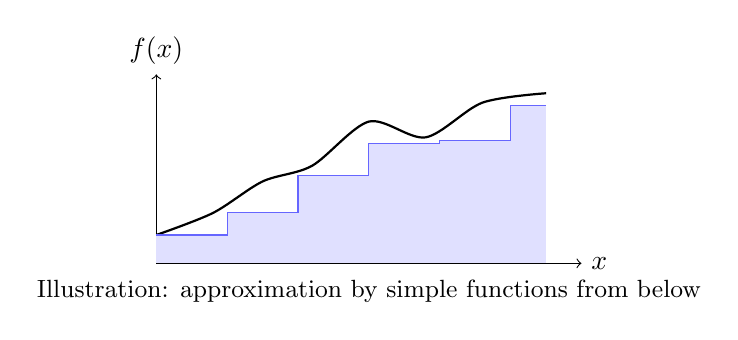
\begin{tikzpicture}[x=0.9cm,y=0.8cm]
 \draw[->] (0,0) -- (6,0) node[right] {$x$};
 \draw[->] (0,0) -- (0,3) node[above] {$f(x)$};
 \draw[thick] plot[smooth] coordinates{(0,0.45)(0.8,0.8)(1.5,1.3)(2.2,1.55)(3,2.25)(3.8,2)(4.6,2.55)(5.5,2.7)};
 \fill[blue!12] (0,0) rectangle (1,0.45);
 \fill[blue!12] (1,0) rectangle (2,0.8);
 \fill[blue!12] (2,0) rectangle (3,1.4);
 \fill[blue!12] (3,0) rectangle (4,1.9);
 \fill[blue!12] (4,0) rectangle (5,1.95);
 \fill[blue!12] (5,0) rectangle (5.5,2.5);
 \draw[blue!60] (0,0.45)--(1,0.45)--(1,0.8)--(2,0.8)--(2,1.4)--(3,1.4)--(3,1.9)--(4,1.9)--(4,1.95)--(5,1.95)--(5,2.5)--(5.5,2.5);
 \node[font=\small] at (3,-0.45) {Illustration: approximation by simple functions from below};
\end{tikzpicture}
\end{center}
\begin{proposition}[Monotone convergence theorem]
If $0\le f_1\le f_2\le\cdots$ are measurable and $f_n\uparrow f$ pointwise, then
\[
\int_S f_n\,d\mu\uparrow\int_S f\,d\mu.
\]
\end{proposition}
We use this theorem without reproducing its full proof. It allows limits of increasing nonnegative functions to pass through the integral.


\subsection*{Integral lower sums and simple approximations}
The use of simple functions corresponds closely to the partition-based intuition in the original notes. Given a finite measurable partition $S=A_1\mathbin{\dot\cup}\cdots\mathbin{\dot\cup}A_m$, choose nonnegative numbers $a_i\le \inf_{s\in A_i}f(s)$ (when the infimum is well defined). The simple function $s=\sum_i a_i\mathbf1_{A_i}$ then satisfies $0\le s\le f$, and its integral is
\[
\int_S s\,d\mu=\sum_{i=1}^{m}a_i\mu(A_i).
\]
Taking the supremum over such lower approximations recovers the Lebesgue integral for nonnegative measurable $f$. Unlike a Riemann partition, a measurable partition need not consist of neighboring intervals. It may group together points according to the \emph{value} of the function, providing much more flexibility for discontinuous functions.

For instance, when $f=3\mathbf1_A+2\mathbf1_{S\setminus A}$ and $\mu(S)<\infty$, $f$ is already simple and
\[
\int_S f\,d\mu=3\mu(A)+2\mu(S\setminus A).
\]
This demonstrates explicitly how integrating a simple function reduces to summing measured contributions.

\section*{4. Signed integrals and dominated convergence (\S4.3)}
For a real-valued measurable function $f$, let
\[
f_+=\max\{f,0\},\qquad f_-=\max\{-f,0\},\qquad f=f_+-f_-.
\]
The integral is defined by $\int f\,d\mu=\int f_+\,d\mu-\int f_-\,d\mu$ whenever the difference is defined. It is \emph{integrable} when
\[
\int_S|f|\,d\mu<\infty.
\]
For integrable $f,g$ and real scalars $a,b$, the integral is linear:
$\int(af+bg)\,d\mu=a\int f\,d\mu+b\int g\,d\mu$.
Moreover, if $f\le g$ almost everywhere, then $\int f\,d\mu\le\int g\,d\mu$ (provided the integrals exist), and
\[
\left|\int_S f\,d\mu\right|\le\int_S|f|\,d\mu.
\]

\begin{proposition}[Dominated convergence theorem]
If the measurable functions $f_n$ converge to $f$ almost everywhere and there is a \emph{single integrable} function $g\ge0$ satisfying $|f_n|\le g$ almost everywhere for every $n$, then $f$ is integrable and
\[
\lim_{n\to\infty}\int_S f_n\,d\mu=\int_S f\,d\mu.
\]
\end{proposition}
The one-sided inequality $f_n<g$ alone is \emph{not} sufficient. The same integrable majorant must control the absolute values of the entire sequence.

\subsection*{Example: Lebesgue but not Riemann integrable}
On $[0,1]$, consider $f(x)=\mathbf1_{[0,1]\setminus\Q}(x)$, equal to one at irrational numbers and zero at rational numbers. Both rationals and irrationals are dense in every subinterval; hence every nontrivial Riemann partition has lower sum zero and upper sum one. The function is therefore not Riemann integrable. As the rationals form a countable set of Lebesgue measure zero,
\[
\int_{[0,1]}f(x)\,dx=1.
\]


\subsection*{Why domination matters}
Pointwise convergence does not generally allow one to swap the order of a limit and an integral. On the probability space $([0,1],\mathcal B([0,1]),\lambda)$, set
\[
f_n(x)=n\,\mathbf1_{(0,1/n)}(x).
\]
Then $f_n(x)\to0$ for each fixed $x\in[0,1]$, but
\[
\int_0^1 f_n(x)\,dx=n\frac1n=1
\quad\text{for every }n.
\]
Thus $\lim_n\int f_n\,d\lambda=1$ while $\int\lim_n f_n\,d\lambda=0$. There is no common integrable bound on the sequence. This illustration makes clear why the correct hypotheses of dominated convergence are substantial rather than cosmetic.

The example $\mathbf1_{[0,1]\setminus\Q}$ shows a separate point: Riemann integrability and Lebesgue integrability have different domains. Every subinterval contains rational and irrational numbers, so its upper and lower Riemann sums differ. Yet the complement of the rationals occupies all the Lebesgue measure in $[0,1]$, and its Lebesgue integral is one.

\section*{5. Expectation (\S4.4)}
For an integrable real random variable $X$ on $(\Omega,\mathcal A,P)$, its expectation is
\[
\E X=\int_\Omega X\,dP.
\]
The properties of the Lebesgue integral immediately give linearity $\E(aX+bY)=a\E X+b\E Y$, monotonicity ($X\le Y\implies\E X\le\E Y$ for integrable variables), and $|\E X|\le\E|X|$.

\subsection*{Convergence theorems for expectation}
\begin{itemize}[leftmargin=*]
\item \textbf{Dominated convergence.} If $X_n\to X$ almost surely and $|X_n|\le Y$ almost surely for all $n$, where $Y\ge0$ and $\E Y<\infty$, then $\E X_n\to\E X$.
\item \textbf{Bounded convergence on a probability space.} If $X_n\to X$ almost surely and $|X_n|\le C$ for one finite constant $C$ and all $n$, then $\E X_n\to\E X$.
\item \textbf{Monotone convergence.} If $0\le X_n\uparrow X$ almost surely, then $\E X_n\uparrow\E X$, with the possibility of $+\infty$.
\end{itemize}
Individual integrability of the $X_n$ is not enough by itself to exchange expectation with the limit.


\subsection*{Expectation from laws rather than sample outcomes}
If $X$ is integrable and has law $\mu_X$ on $\R$, then
\[
\E X=\int_{\Omega}X(\omega)\,P(d\omega)
=\int_{\R}x\,\mu_X(dx).
\]
More generally, for a measurable real function $h$ with $\E|h(X)|<\infty$,
\[
\E[h(X)]=\int_{\R}h(x)\,\mu_X(dx).
\]
The identity illustrates why the law is so useful: to compute expectations of observables, it is often enough to know the distribution and not the details of the original experiment. When moving from convergence of distributions to convergence of expectations, however, one must still check the relevant moment or uniform-integrability conditions.

\section*{Reading note}
The distinction between pointwise or almost-sure convergence and convergence of integrals becomes important later, when probability laws and second moments are passed to limits in the Wasserstein argument.
\end{document}
